\chapter{Análisis de Fourier}

En el curso Física Matemática I ya se discutió el estudio de la Serie de Fourier. En este curso, haremos un rápido resumen de dichos contenidos, pues son la base para introducir el concepto de la \emph{transformada de Fourier}, que será de utilidad para la resolución de algunas ecuaciones diferenciales parciales cuyas condiciones de borde son periódicas.

\section{Periodicidad y paridad de funciones}

% \subsection{Funciones periódicas}

\begin{defi} \marginnote{Función periódica}
Una función $f: \mathbb{R} \to \mathbb{C} $ se dice que es \textbf{periódica de período} $T$, con $T\neq 0$, si 
\begin{equation} \label{Periodica}
    \boxed{
f(t) = f(t + T), \quad \forall \ t \in \mathbb{R}.}    
\end{equation}



La constante $T$ la tomaremos como la  menor constante positiva que satisface la igualdad \eqref{Periodica}.
\end{defi}


\begin{propiedad} 
    \textbf{Propiedades de las funciones periódicas.}
    \begin{enumerate}
        \item Si $f$ es periódica de periodo $T$, entonces $$f(t) = f(t + nT), \quad n = 0, \pm 1, \pm 2, \dots$$
        
        \item Si $f(t)$ y $g(t)$ son funciones periódicas de período $T$, entonces la función
        $$h(t) = \alpha f(t) + \beta g(t); \quad \alpha, \beta \in \mathbb{C},$$
        tiene el mismo período $T$.
    
        \item En general, si la función 
        $$f(t) = \cos (\omega_1 t) + \cos (\omega_2 t)$$
        es periódica de período $T$, entonces es posible encontrar dos enteros $n$ y $m$ tales que 
        \begin{align}
            \omega_1 T &= 2\pi n,  \label{Periodica1}\\
             \omega_2 T &= 2\pi m. \label{Periodica2}
        \end{align}
        
        El cociente de \eqref{Periodica1} y \eqref{Periodica2} es
        $$\frac{\omega_1}{\omega_2} = \frac{n}{m} \ ,$$
        es decir, la relación $\omega_1/ \omega_2$ debe ser un número racional.
    \end{enumerate}
\end{propiedad}


\begin{ejemplo}
Encuentre el período de la función $f(t) = \cos \left(\frac{t}{3}\right) + \cos \left(\frac{t}{4}\right)$.

\textbf{Solución:} Si la función $f(t)$ es periódica con período $T$, entonces, de \eqref{Periodica},
$$\cos \frac{1}{3}(t + T) + \cos \frac{1}{4}(t + T) = \cos \frac{t}{3} + \cos \frac{t}{4}.$$

Como $\cos(\theta + 2\pi n) = \cos \theta, n \in \mathbb{Z}$, obtenemos que 
$$\frac{1}{3} T = 2\pi n, \quad \frac{1}{4}T = 2\pi m; \quad n,m \in \mathbb{Z}.$$

Por consiguiente $T = 6\pi n = 8\pi m$; cuando $n = 4$ y $m=3$, se obtiene el mínimo valor de $T$. Así, $T = 24\pi$.
\end{ejemplo}

\begin{defi} \marginnote{Función seccionalmente continua}
    Una función $f: [a,b] \longrightarrow \mathbb{C}$ es \textbf{seccionalmente continua} si $[a,b]$ tiene una partición finita $a = t_0 < t_1 < \cdots < t_n = b$ tal que $f$ es continua y acotada en cada intervalo abierto $(t_i, t_{i+1}), i = 0, \dots, n-1$.
    
    Denotaremos por $\mathscr{C}[a,b]$ al conjunto de las funciones complejas seccionalmente continuas.
\end{defi}


\begin{propo}
Sea $f: \mathbb{R} \longrightarrow \mathbb{C}$ una función periódica de período $T$. Sea $a \in \mathbb{R}$, entonces
$$ \int_{a-T/2}^{a + T/2} f(t) \,dt = \int_{- T/2}^{T/2} f(t) \,dt .$$
\end{propo}

\begin{demo}
Utilizando la propiedad de aditividad de las integrales,
\begin{equation*}
    \int_{a-T/2}^{a + T/2} f(t) \,dt = \int_{a - T/2}^{-T/2} f(t) \,dt + \int_{- T/2}^{a + T/2} f(t) \,dt.
\end{equation*}

Haciendo la sustitución  $t = t' - T ~\Rightarrow~ dt = dt'$ en la primera integral, obtenemos
\begin{align*}
   \int_{a - T/2}^{-T/2}f(t) \,dt + \int_{- T/2}^{a + T/2} f(t) \,dt   &= \int_{a + T/2}^{T/2} f(t'-T) \,dt' + \int_{- T/2}^{a + T/2} f(t) \,dt \\
   &= \int_{a + T/2}^{T/2} f(t'-T + T) \,dt' + \int_{- T/2}^{a + T/2} f(t) \,dt \\
   &= \int_{a + T/2}^{T/2} f(t') \,dt' + \int_{-T/2}^{a + T/2} f(t) \,dt \\
   &= \int_{-T/2}^{T/2} f(t) \,dt.
\end{align*}
\end{demo}

\begin{defi}\marginnote{Extensión periódica}
Sea $f: [a,b] \rightarrow \mathbb{R}$ seccionalmente continua, se llama \textbf{extensión periódica} de $f$ a la función $f_e: \mathbb{R} \rightarrow \mathbb{R}$,
\begin{equation} 
    \boxed{f_e(t) = f(t + k_0 (b-a))} \ , 
\end{equation}
donde $k_0 \in \mathbb{Z}$ es el único entero que verifica $t + k_0(b-a) \in [a,b].$
\end{defi}

\begin{ejemplo}
La extensión periódica de $f \in \mathscr{C}[-\pi,\pi]$ real es
$$f_e(t) = f_e(t + 2\pi)$$

\begin{figure}[H]
    \centering
    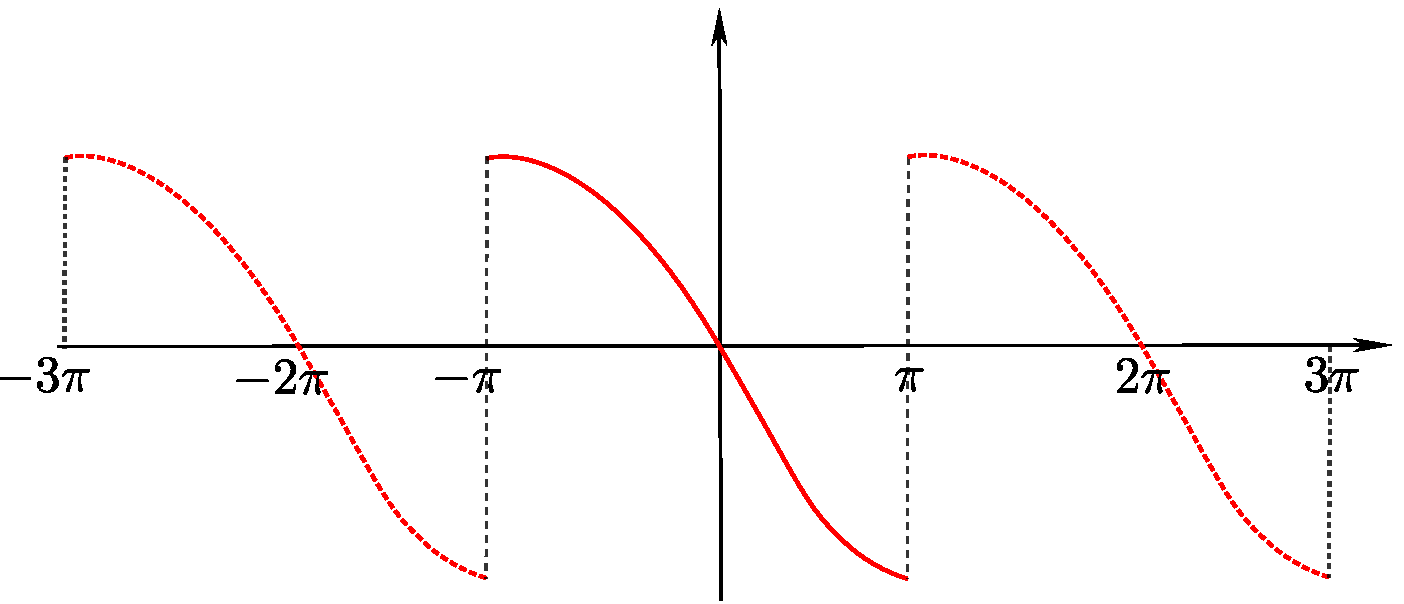
\includegraphics[scale = 0.45]{Figuras/Periocidad.pdf}
    \caption{Extensión periódica de una función real seccionalmente continua en $[-\pi,\pi]$.}
\end{figure}
\end{ejemplo}

% \subsection{Funciones pares e impares}
 
\begin{defi} \marginnote{Funciones pares e impares}
Sea $f: [-a,a] \longrightarrow \mathbb{R}$ perteneciente a $\mathscr{C}[-a,a]$.
Diremos que $f$ es una \textbf{función par} si y solo si, para todo $x$ en el intervalo $[-a,a]$, se cumple que
\begin{equation}
    f(-t) = f(t) \ .
\end{equation}
De forma similar, diremos que $f$ es una \textbf{función impar} si y solo si, para todo $x$ en el intervalo $[-a,a]$, se cumple que
\vspace{-0.1cm}
\begin{equation}
     f(-t) = -f(t) \ .
\end{equation}
\end{defi} 

\begin{propo}
    Sea $f: [-a,a] \longrightarrow \mathbb{R}$ integrable,
    \begin{align*}
        f ~\mbox{es par} &\Rightarrow \int_{-a}^a f(t) \,dt = 2 \int_0^a f(t) \,dt. \\
        f ~\mbox{es impar} &\Rightarrow \int_{-a}^a f(t) \,dt = 0.
    \end{align*}
\end{propo}

\begin{obs}{Observación}
    Toda función $f:[-a,a] \longrightarrow \mathbb{R}$ puede expresarse como la suma de una función par más otra impar: $f = f_p + f_i$ con 
    \begin{equation*}
        f_p(t) = \frac{f(t) + f(-t)}{2}, \quad f_i(t) = \frac{f(t) - f(-t)}{2} \ .
    \end{equation*}
\end{obs}

\begin{defi} \marginnote{Extensión par e impar}
Sea $f \in \mathscr{C}[0,a]$ real, entonces la \textbf{extensión par} y la \textbf{extensión impar} de $f$ están definidas, respectivamente, por:
\begin{equation*}
    E_f(t) = \left\{ \begin{array}{cll}
    f(-t)     & \mbox{si} & -a \leq t < 0 \\
    f(t)     & \mbox{si} & 0 \leq t \leq a
    \end{array} \right. , ~ O_f(t) = \left\{ \begin{array}{cll}
    -f(-t)     & \mbox{si} & -a \leq t < 0 \\
    f(t)     & \mbox{si} & 0 \leq t \leq a
    \end{array} \right. .
\end{equation*}
Ambas extensiones se encuentran definidas en el intervalo $[-a,a]$.
\end{defi}

\begin{figure}[H]
    \centering
    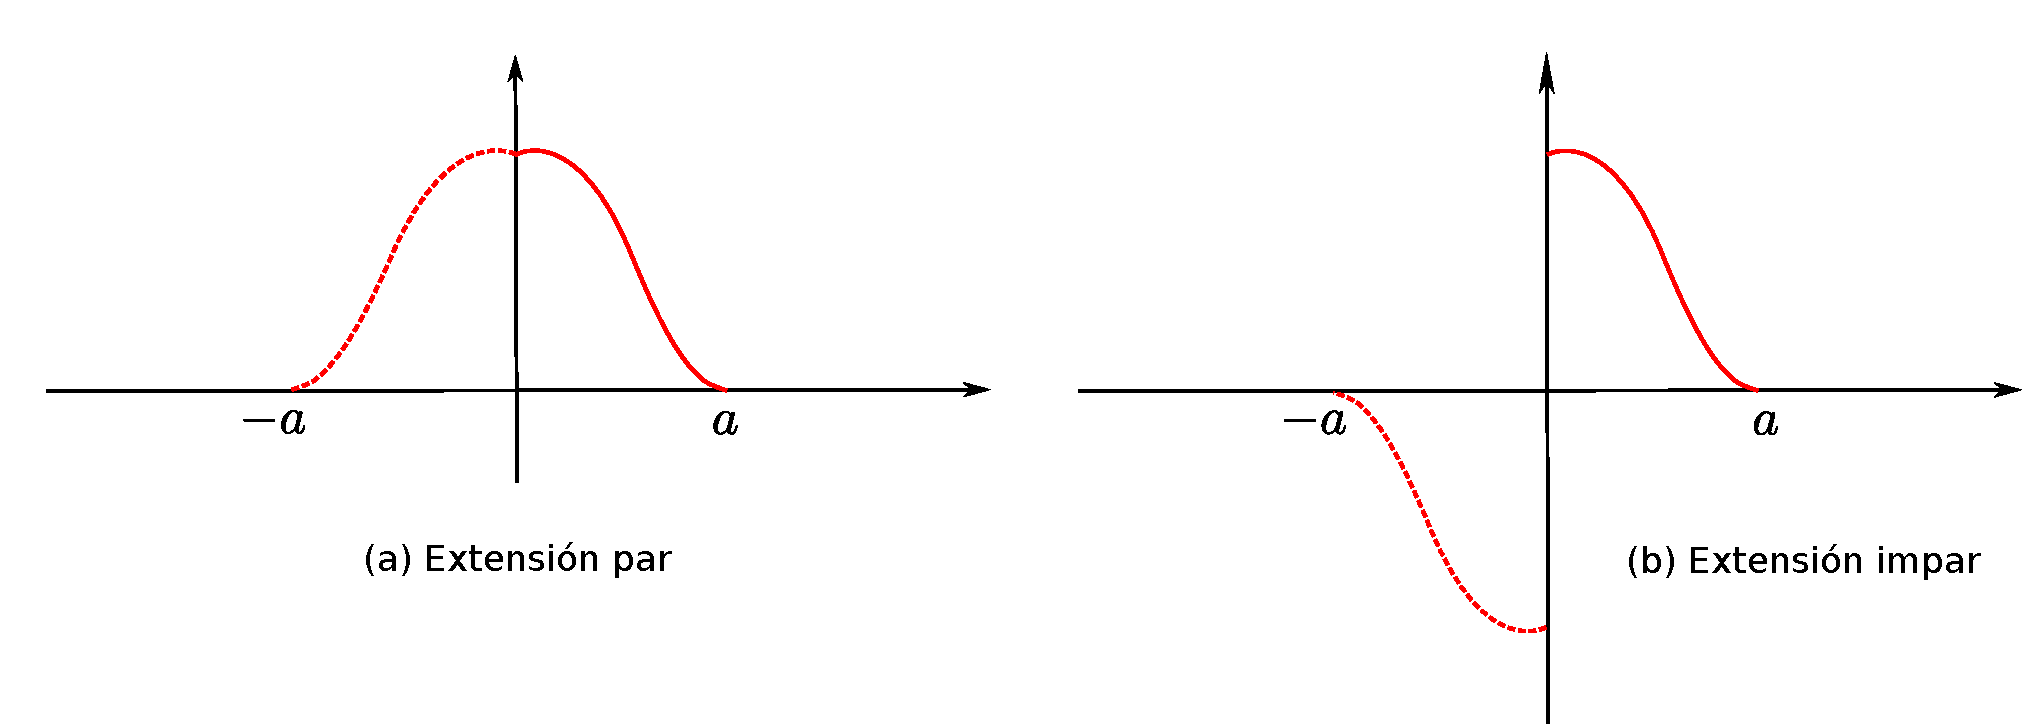
\includegraphics[width = \textwidth]{Figuras/Paridad.pdf}
    \caption{Extensión par e impar de una función real seccionalmente continua en $[0,a]$. }
\end{figure}

\section{Serie de Fourier trigonométrica}

% \subsection{Definición}

\begin{propo}
    En el espacio $\mathscr{C}[a,b]$, el conjunto formado por las funciones
    $$\left\{ 1, \cos\left( \frac{2n \pi}{T}x \right), \sin\left( \frac{2n \pi}{T}x \right) \right\}_{n=1}^{\infty}$$
    es un conjunto ortogonal, con $T = b-a$ el periodo de la función.
\end{propo}


\begin{defi} \marginnote{Sistema trigonométrico}
    Llamamos \textbf{sistema trigonométrico} al conjunto de funciones ortonormales en el espacio $\mathscr{C}[-\pi,\pi]$, definido como
    $$\left\{ \frac{1}{\sqrt{2\pi}}, \frac{\cos(nt)}{\sqrt{\pi}}, \frac{\sin(nt)}{\sqrt{\pi}} \right\}_{n=1}^{\infty}$$
\end{defi}

\begin{defi} \marginnote{Condiciones de Dirichlet}
    Una función $f$ satisface las llamadas \textbf{Condiciones de Dirichlet} si satisface
    \begin{enumerate}
        \item Se encuentra definida en un intervalo $(a,a+T)$.
        \item Tanto $f$ como su derivada son funciones seccionalmente continuas en el intervalo $(a,a+T)$.
        \item $f$ tiene un número finito de discontinuidades \emph{finitas}.
        \item $f$ es una función periódica de periodo $T$.
    \end{enumerate}

\end{defi}

\begin{defi} \marginnote{Serie de Fourier}
Sea $f \in \mathscr{C}[a, a+T]$ una función que satisface las condiciones de Dirichlet. Entonces, ella puede ser aproximada por la serie 
\begin{equation}
    \frac{a_0}{2} + \sum_{n=1}^{\infty} \left( a_n \cos\left( \frac{2n\pi}{T}x \right) + b_n \sin\left( \frac{2n\pi}{T}x \right) \right) \approx f(x) \ . \label{FourierTrigo}
\end{equation}

Esta expansión se denomina \textbf{serie trigonométrica de Fourier} o simplemente \textbf{serie de Fourier}, donde los \textit{coeficientes de Fourier} están dados por:
\begin{align*}
    a_0 &= \frac{2}{T} \int_{a}^{a+T} f(t) \,dt, \\
    a_n &= \frac{2}{T} \int_{a}^{a+T} f(t) \cos\left( \frac{2n\pi}{T}t \right) \,dt, \quad n = 1,2, \dots\\
    b_n &= \frac{2}{T} \int_{a}^{a+T} f(t) \sin\left( \frac{2n\pi}{T}t \right) \,dt. \quad n = 1,2, \dots
\end{align*}
\end{defi}

\begin{ejemplo} \label{EjemploFourier1}
    Consideremos la función $f(x) = x^2$ definida para $x\in [-\pi,\pi]$, la cual es continua con derivada $f'(x) = 2x$ también continua, luego la serie de Fourier de $f$ converge puntualmente a $f$ para todo $x \in (-\pi,\pi)$. Para los extremos $x = \pm \pi$ vemos que $f(\pi) = f(-\pi)$, por lo tanto la serie converge puntualmente a $f$ para todo $x \in [-\pi,\pi]$.
    
    Sus coeficientes de Fourier están dados por:
    \begin{align*}
        a_0 &= \frac{1}{\pi} \int_{-\pi}^{\pi} x^2 \,dx = \left. \frac{x^3}{3\pi} \right|_{-\pi}^{\pi} = \frac{2}{3} \pi^2, \\
        a_n &= \frac{1}{\pi} \int_{-\pi}^{\pi} x^2 \cos(n x)\,dx =   \left. \frac{1}{n\pi} x^2 \sin(nx)  \right|_{-\pi}^{\pi} - \frac{2}{n\pi} \int_{-\pi}^{\pi} x \sin(nx) \,dx\\
        &= \left.   \frac{2}{n^2\pi} x \cos(nx)\right|_{-\pi}^{\pi} - \frac{2}{n^2 \pi} \cancelto{0}{\int_{-\pi}^{\pi} \cos(nx) \,dx }\\
        &=  \frac{4}{n^2} \cos(n\pi) =  (-1)^n \frac{4}{n^2}, \quad n = 1,2,\dots\\
         b_n &= \frac{1}{\pi} \int_{-\pi}^{\pi} x^2 \sin(nx)\,dx = 0, \quad n = 1,2, \dots
    \end{align*}
    
    Entonces, su serie de Fourier es
    \begin{equation}
    f(x) = \frac{\pi^2}{3} + \sum_{n=1}^{\infty} (-1)^n \frac{4}{n^2} \cos(nx), \qquad x \in [-\pi,\pi].    \label{FourierCuadratica}
    \end{equation}
    
    Es claro que la serie de Fourier de $f(x) = x^2$ para todo $x\in \mathbb{R}$ representa la extensión periódica de los valores de $f(x)$ en el intervalo $[-\pi,\pi]$.
    
    La gráfica de $f$ en conjunto con diferentes sumas parciales de su serie de Fourier están representadas en la figura \ref{fig:EjemploFourier1}. 
    
    % \begin{figure}[htb]
        \centering
        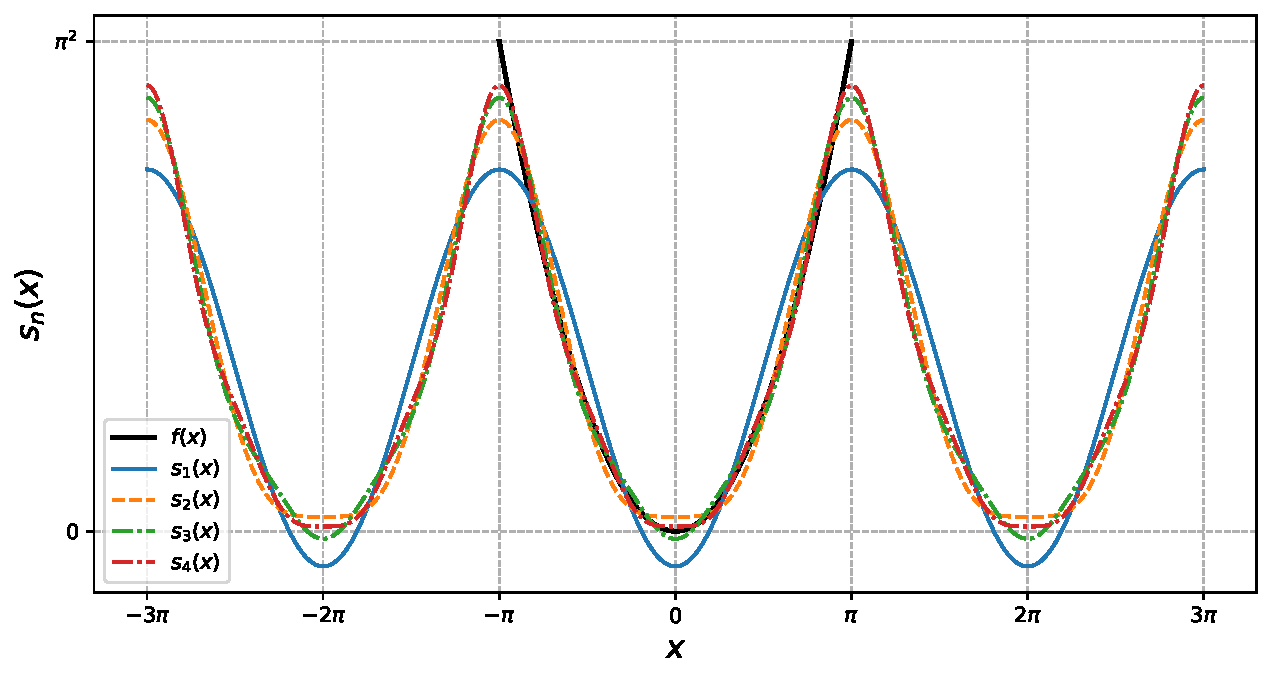
\includegraphics[width = 0.8\textwidth]{Figuras/EjemploFourier1.pdf}
        \captionof{figure}{Serie de Fourier de la función $f(x) = x^2, -\pi \leq x \leq \pi$, truncada hasta $n = 4$.}
        \label{fig:EjemploFourier1}
    % \end{figure}
    % El teorema visto para convergencia uniforme nos garantiza que esta serie converge uniformemente a $f(x) = x^2$ en $[-\pi,\pi]$, es más, al aplicar el criterio de M de Weierstrass a la serie, ésta converge para todo $x \in \mathbb{R}$, pues
    % $$\forall  x \in \mathbb{R}: ~ \left|(-1)^n \frac{4}{n^2} \cos(nx)\right| \leq \frac{4}{n^2} = M_n ~~\mbox{y}~~  \sum\limits_{n=1}^{\infty} M_n < \infty.$$
\end{ejemplo}

% \textbf{Observación}: La serie de Fourier de $f$ converge en media a $f$, o sea, 
% \begin{shaded}
% $$f(t) \sim \frac{a_0}{2} + \sum_{n=1}^{\infty} (a_n \cos(nt) + b_n \sin(nt)).$$    
% \end{shaded}

% \begin{propo} \label{C.FourierCero}
% Los coeficientes de la serie trigonométrica de Fourier de $f \in \mathscr{C}[-\pi,\pi]$ convergen a cero cuando $n \to \infty$, es decir,
% $$\lim_{n \to + \infty} a_n = \lim_{n \to + \infty} b_n = 0.$$
% \end{propo}

% \begin{demo}
% Si denotamos el sistema trigonométrico por 
% $$\varphi_0(t) = \frac{1}{\sqrt{2\pi}}, ~ \varphi_{2n-1}(t) = \frac{1}{\sqrt{\pi}} \cos(nt), ~ \varphi_{2n(t)} = \frac{1}{\sqrt{\pi}} \sin(nt), \quad n = 1,2, \dots$$

% tenemos que la serie generalizada de Fourier queda
% $$\sum_{n=0}^{\infty} C_n \varphi_n(t) = C_0 \varphi_0(t) + \sum_{n=1}^{\infty} \left[ C_{2n-1} \varphi_{2n-1}(t) + C_{2n} \varphi_{2n}(t) \right] ,$$

% la cual corresponde a la serie trigonométrica de Fourier de $f \in \mathscr{C}[-\pi,\pi]$, donde 
% $$a_0 = \sqrt{\frac{2}{\pi}} C_0, ~ a_n = \frac{C_{2n-1}}{\sqrt{\pi}}, ~ b_n = \frac{C_{2n}}{\sqrt{\pi}}, \quad n = 1,2, \dots$$

% De lo discutido en el primer capítulo, una de las consecuencias de la desigualdad de Bessel \eqref{D.Bessel} es que 
% $$\lim_{n \to + \infty} C_n = \lim_{n \to + \infty} \langle f, \varphi_n \rangle = 0 ~\Rightarrow~ \lim_{n \to \infty} C_{2n-1} = \lim_{n \to \infty} C_{2n} = 0. $$

% Por lo tanto, 
% $$\lim_{n \to + \infty} a_n = \lim_{n \to + \infty} b_n = 0.$$

% \end{demo}

% ¿Convergerá puntual y/o uniformemente la serie de Fourier a $f(t)$? ¿Qué condiciones deben cumplirse?

% Antes de responder estas preguntas, primero justifiquemos que es suficiente trabajar con funciones a valores reales, a pesar de que los siguientes teoremas también son válidos para funciones a valores complejos. 

\subsection{Serie de Fourier de una función compleja de variable real}

Sea $f = u + iv \in \mathscr{C}[a,b]$, su serie de Fourier trigonométrica está dada por \eqref{FourierTrigo} con 
\begin{align*}
    a_0 &= \frac{2}{T} \int_{a}^{b} f(t) \,dt =  \frac{2}{T} \int_a^b u(t) \,dt + i\frac{2}{T} \int_a^b v(t) \,dt,\\
    a_n &= \frac{2}{T} \int_a^b f(t) \cos\left( \frac{2n\pi}{T}t \right) \,dt = \frac{2}{T} \int_a^b u(t) \cos\left( \frac{2n\pi}{T}t \right) \,dt + i\frac{2}{T} \int_a^b v(t) \cos\left( \frac{2n\pi}{T}t \right) \,dt , \quad n \in \mathbb{N} \\
    b_n &= \frac{2}{T} \int_a^b f(t) \sin\left( \frac{2n\pi}{T}t \right) \,dt = \frac{2}{T} \int_a^b u(t) \sin\left( \frac{2n\pi}{T}t \right) \,dt + i\frac{2}{T} \int_a^b v(t) \sin\left( \frac{2n\pi}{T}t \right) \,dt, \quad n \in \mathbb{N}
\end{align*}

Entonces, su serie de Fourier nos queda
\begin{align}
  f(t) & \sim   \left\{ \frac{\real(a_0)}{2} + \sum_{n=1}^{\infty} \left[ \real(a_n) \cos\left( \frac{2n\pi}{T}t \right) + \real\left( b_n \right) \sin\left( \frac{2n\pi}{T}t \right) \right] \right\}  \nonumber \\
   & \qquad + i \left\{ \frac{\im(a_0)}{2} + \sum_{n=1}^{\infty} \left[\im(a_n) \cos\left( \frac{2n\pi}{T}t \right) + \im(b_n) \sin\left( \frac{2n\pi}{T}t \right) \right] \right\},
\end{align}

es decir, la serie de Fourier de $f = u + iv$ será dada por
\begin{equation}
    S_F(f) = S_F(u) + i S_F(v) \ ,
\end{equation}
donde $S_F$ representa a una serie de Fourier.


\subsection{Series de senos y cosenos}

\begin{defi} \marginnote{Serie de Fourier seno y serie de Fourier coseno}
    Dadas las extensiones par e impar de una función, $E_f, O_f: [a,b] \to \mathbb{R}$, es posible obtener el desarrollo en serie de Fourier de cada una de estas, que corresponden a los \textbf{desarrollos en serie de Fourier de coseno y de seno} de $f$, respectivamente. Estos son definidos como
    \begin{align*}
        E_f(t) & \sim \frac{a_0}{2}  + \sum_{n=1}^{\infty} a_n \cos\left( \frac{2n\pi}{T}t \right), & ~~\mbox{donde}~~ a_n = \frac{2}{T} \int_a^{b} f(t) \cos\left( \frac{2n\pi}{T}t \right)  dt \ , \\
        O_f(t) & \sim  \sum_{n=1}^{\infty} b_n \sin\left( \frac{2n\pi}{T}t \right), & ~~\mbox{donde} ~~ b_n = \frac{2}{T} \int_a^{b} f(t) \sin\left( \frac{2n\pi}{T}t \right) \ dt \ .
    \end{align*}

    En ambos casos, se ha hecho uso de las propiedades de las funciones pares e impares para hallar los coeficientes de las series.
\end{defi}

% Puesto que $E_f, O_f: [-\pi,\pi] \to \mathbb{R}$ son seccionalmente continuas, se puede obtener el desarrollo en serie de Fourier de estas, los cuales están definidos por: \footnote{La forma de las series seno y coseno, con sus respectivos coeficientes, se obtienen al aplicar las propiedades vistas para las funciones pares e impares.}
% $$ 

% y
% $$ .$$

% Estos son llamados \textbf{desarrollos en serie de Fourier de coseno y de seno de $f$}, respectivamente.

% \subsection{Convergencia puntual y uniforme}

% \begin{defi}
% Sea $f: [a,b] \longrightarrow \mathbb{R}$, para $t_0 \in [a,b]$ definimos
% \begin{align*}
%     f(t_0^+) &= \lim_{t \to t_0^+} f(t), \\
%     f(t_0^-) &= \lim_{t \to t_0^-} f(t),
% \end{align*}

% si existen los límites. 

% Una discontinuidad en $t_0$ tal que $f(t_0^+)$ y $f(t_0^-)$ existen se denomina \textbf{discontinuidad de salto} y $f(t_0^+) - f(t_0^-)$ recibe el nombre de \textbf{salto} de $f$ en $t_0$.
% \end{defi}

% \textbf{Observaciones:} 

% \begin{enumerate}
%     \item La magnitud del salto es $|f(t_0^+) - f(t_0^-)|$.
    
%     \item El salto se anula cuando $f(t_0) = f(t_0^+) = f(t_0^-)$, es decir, cuando $f$ es continua en $t_0$.
    
%     \item Una función $f: [a,b] \longrightarrow \mathbb{R}$ seccionalmente continua tiene discontinuidades de salto.
% \end{enumerate}

% \begin{defi}
% Sea $f:[a,b] \longrightarrow \mathbb{R}$, con una discontinuidad de salto en $t_0 \in [a,b]$, definimos la \textbf{derivada por la derecha} como 
% $$f'(t_0^+) = \lim_{h \to 0^+} \frac{f(t_0 + h ) - f(t_0^+)}{h}$$

% cuando el límite existe. Similarmente, definimos la \textbf{derivada por la izquierda} como 
% $$f'(t_0^-) = \lim_{h \to 0^-} \frac{f(t_0 + h ) - f(t_0^-)}{h}$$

% cuando el límite existe.
% \end{defi}

% \begin{teorema}[Convergencia puntual de la serie de Fourier] \label{Puntual}
% Sea $f(t)$ una función real seccionalmente continua en el intervalo $-\pi < t < \pi$. Su serie de Fourier trigonométrica converge al valor medio
% \vspace{-0.05cm}
% $$\frac{f(t^+) + f(t^-)}{2}$$

% para cada $t \in (-\pi,\pi)$ donde ambas derivadas laterales $f'(t^+)$ y $f'(t^-)$ existen.
% \end{teorema}

% \textbf{Observación:} Si denotamos por $f_e$ a la extensión periódica de $f$, a partir del teorema anterior, la expansión en serie de Fourier converge a $f_e$ para todo $x \in \mathbb{R}$ al extenderla periódicamente al valor medio
% $$\frac{f_e(t^+) + f_e(t^-)}{2}.$$

% De hecho, en los extremos $t = \pm \pi$, la serie converge a 
% $$\frac{f(-\pi^+) + f(\pi^-)}{2}.$$

% En efecto, observemos que
% $$f_e(-\pi^+) = f(-\pi^+) ~~\mbox{y}~~ f_e(-\pi^-) = f(\pi^-).$$

% Luego, el cociente
% $$\frac{f_e(-\pi^+) + f_e(-\pi^-)}{2} = \frac{f(-\pi^+) + f(\pi-)}{2}.$$

% Análogamente para $t = \pi$.

% \begin{teorema}[Convergencia uniforme] \label{C.Uniforme}
% Supóngase que $f$ es continua en $[-\pi,\pi]$, $f(-\pi) = f(\pi)$ y que $f'$ es continua por tramos, con discontinuidades de salto. Entonces la serie de Fourier trigonométrica de $f$ converge a $f$ absolutamente y uniformemente.
% \end{teorema}

% \subsection{Ejemplos}



% Podemos usar la expansión en serie de Fourier de $f(x) = x^2$ en $[-\pi,\pi]$ para probar que 
% $$\sum_{n=1}^{\infty} \frac{1}{n^2} = 1 + \frac{1}{4} + \frac{1}{9} + \cdots = \frac{\pi^2}{6}.$$

% En efecto, al evaluar $x = \pi$ en \eqref{FourierCuadratica}, obtenemos que 
% $$f(\pi) = \frac{\pi^2}{3} + \sum_{n=1}^{\infty} (-1)^n \frac{4}{n^2} \cos(n\pi) = \frac{\pi^2}{3} + \sum_{n=1}^{\infty} (-1)^{2n} \frac{4}{n^2} = \frac{\pi^2}{3} +  \sum_{n=1}^{\infty} \frac{4}{n^2}.$$

% Así,
% $$\pi^2 = \frac{\pi^2}{3} + 4 \sum_{n=1}^{\infty} \frac{1}{n^2} \Rightarrow \sum_{n=1}^{\infty} \frac{1}{n^2} = \frac{\pi^2}{6}.$$

\begin{ejemplo} \label{Signo}
Consideremos la función signo  definida por
$$f(x) := \left\{ \begin{array}{cc}
     -1,& - \pi \leq x < 0  \\
     1,&   0 \leq x \leq \pi
\end{array} \right. .$$

La función es seccionalmente continua con $x = 0$ punto de discontinuidad de salto y las derivadas laterales existen para todo $x \in (-\pi,\pi)$, luego la serie de Fourier de $f$ converge puntualmente a $f$ en los puntos de continuidad y a 
$$\frac{f(0^-) + f(0^+)}{2} = 0, \quad \mbox{en} ~ x = 0 ~~\mbox{y}$$
$$\frac{f(-\pi^+) + f(\pi^-)}{2} = 0, \quad \mbox{en} ~ x = \pm \pi. $$

Sus coeficientes de Fourier están dados por:
\begin{align*}
    a_0 &= \frac{1}{\pi} \int_{-\pi}^{\pi} f(x) \,dx = 0 , \\
    a_n &= \frac{1}{\pi} \int_{-\pi}^{\pi} f(x) \cos(n x)\,dx = 0, \quad n = 1,2,\dots
\end{align*}
\begin{align*}
     b_n &= \frac{1}{\pi} \int_{-\pi}^{\pi} f(x) \sin(nx) \,dx \\
     &= \frac{1}{\pi} \int_{-\pi}^0 (-1) \sin(nx)\,dx + \frac{1}{\pi} \int_{0}^{\pi} (1) \sin(nx) \,dx \\
     &= \left.  \frac{1}{\pi n} \cos(nx) \right|_{-\pi}^0 - \left. \frac{1}{\pi n} \cos(nx) \right|_{0}^{\pi} \\
     &= \frac{2}{\pi n} [1 - (-1)^n] \\
     &= \left\{ \begin{array}{cl}
         0, & n ~\mbox{par}  \\
         \frac{4}{\pi n}, &  n ~\mbox{impar}
     \end{array} \right. .
\end{align*}

Entonces, su serie de Fourier es 
$$f(x) =  \sum_{n ~impar} \frac{4}{\pi n} \sin(nx) = \sum_{k=1}^{\infty} \frac{4}{\pi} \frac{\sin[(2k-1)x]}{ (2k-1)}.$$

\textbf{Aclaración:} Note que a pesar de haber escrito que la función $f$ es igual a la serie, debemos tener en cuenta que en los punto $x = 0$ y $x = \pm \pi$ converge al valor medio del salto de la discontinuidad.

Es claro que la serie de Fourier de $f$ para todo $x\in \mathbb{R}$ representa la extensión periódica de los valores de $f(x)$ en el intervalo $[-\pi,\pi]$.

La gráfica de $f$ en conjunto con diferentes sumas parciales de su serie de Fourier están representadas en la figura \ref{fig:EjemploFourier2}.

\begin{figure}[H]
    \centering
    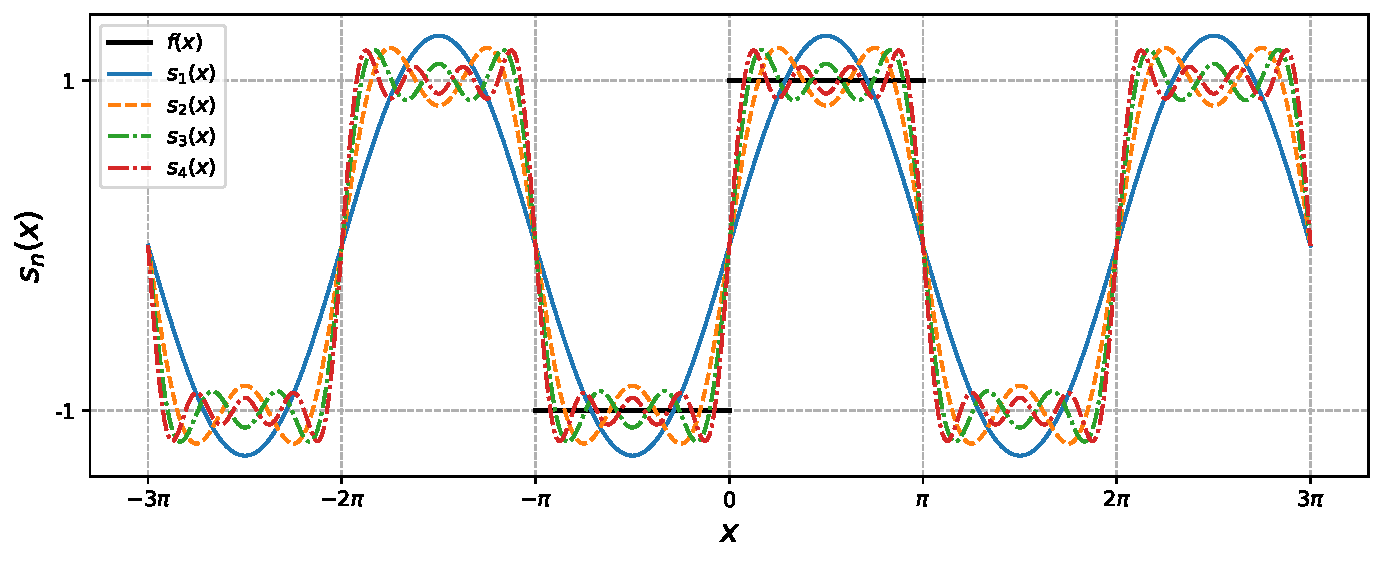
\includegraphics[scale = 0.65]{Figuras/EjemploFourier2.pdf}
    \caption{Serie de Fourier de la función signo truncada hasta $n = 4$.}
     \label{fig:EjemploFourier2}
\end{figure}

\end{ejemplo}

\section{Serie exponencial}

\begin{propo}
    En el espacio $\mathscr{C}[a,a+T]$, el conjunto formado por las funciones 
    \begin{equation}
        \left\{ \frac{1}{\sqrt{T}} \exp\left(i\frac{2n\pi}{T}x\right) \right\}_{n= - \infty}^{n = \infty}
    \end{equation}
    es un conjunto ortonormal.
\end{propo}

\begin{defi} \marginnote{Sistema exponencial}
    Llamamos \textbf{sistema exponencial} al conjunto de funciones ortonormales en el espacio $\mathscr{C}[-\pi,\pi]$, definido como 
    $$\left\{ \frac{1}{\sqrt{2\pi}} e^{int} \right\}_{n= - \infty}^{n = \infty}$$
\end{defi}

\begin{defi} \marginnote{Serie de Fourier exponencial}
Sea $f \in \mathscr{C}[a,a+T]$ una función con un número finito de discontinuidades. Entonces, ella puede ser aproximada por la serie 
\begin{equation}
     \sum_{n=- \infty}^{\infty} c_n \exp\left(i\frac{2n\pi}{T}x\right) \label{FourierExpo}
\end{equation}

Esta expansión se denomina \textbf{serie exponencial de Fourier}  donde los \textit{coeficientes de Fourier} están dados por:
\begin{equation*}
    c_n = \frac{1}{T} \int_{a}^{a+T} f(t) \exp\left(-i\frac{2n\pi}{T}t \right) \ dt \ .
\end{equation*}
\end{defi}

% \textbf{Observación}: La serie de Fourier de $f$ converge en media a $f$, o sea, 
% \begin{shaded}
%  $$f(t) \sim \sum_{n=- \infty}^{\infty} c_n e^{int}.$$   
% \end{shaded}

\begin{propo} \label{TrigoExpo}
La $n$-ésima suma parcial de la serie de Fourier trigonométrica de una función (real o compleja) es igual a la $n$-ésima suma parcial de la serie exponencial.
\end{propo}

\begin{demo}
La $n$-ésima suma parcial de la serie exponencial es
$$ s_n(t) = \sum_{k=-n}^n c_k e^{ikt}.$$

Separando la suma:
\begin{align*}
    s_n(t) &= \sum_{k=-n}^{-1} c_k e^{ikt} + c_0 + \sum_{k=1}^n c_k e^{ikt} \\
    &= c_0 + \sum_{k=1}^n c_k e^{ikt} + \sum_{k=1}^n c_{-k} e^{-ikt} \\
    &= c_0 + \sum_{k=1}^n [c_k e^{ikt} + c_{-k} e^{-ikt}]. 
\end{align*}

Usando la identidad de Euler, $e^{i\theta} = \cos(\theta) + i \sin(\theta)$, encontramos que
$$s_n(t) = c_0 +  \sum_{k=1}^n [(c_k + c_{-k}) \cos(kt) + i(c_k - c_{-k}) \sin(kt)].$$

Desarrollando los coeficientes de la serie exponencial de Fourier, tenemos que
\begingroup
\allowdisplaybreaks
\begin{align*}
    c_0 &= \frac{1}{2\pi} \int_{-\pi}^{\pi} f(t) \,dt, \\
    c_k + c_{-k} &= \frac{1}{2\pi} \int_{-\pi}^{\pi} f(t) e^{-ikt} \,dt + \frac{1}{2\pi} \int_{-\pi}^{\pi} f(t) e^{ikt} \,dt  \\
    &= \frac{1}{2\pi} \int_{-\pi}^{\pi} f(t) [e^{ikt} + e^{-ikt}] \,dt \\
    &= \frac{1}{\pi} \int_{-\pi}^{\pi} f(t) \cos(kt) \,dt; \quad k = 1,2, \dots\\
   i( c_k - c_{-k}) &= \frac{i}{2\pi} \int_{-\pi}^{\pi} f(t) e^{-ikt} \,dt - \frac{i}{2\pi} \int_{-\pi}^{\pi} f(t) e^{ikt} \,dt \\
   &= - \frac{i}{2\pi} \int_{-\pi}^{\pi} f(t) [e^{ikt} - e^{-ikt}] \,dt \\
   &= \frac{1}{\pi} \int_{-\pi}^{\pi} f(t) \sin(kt)\,dt; \quad k = 1,2, \dots
\end{align*}
\endgroup

Comparando las expresiones obtenidas con los coeficientes de la serie de Fourier trigonométrica, podemos concluir que 
$$c_0 = \frac{a_0}{2}, ~  c_k + c_{-k} = a_k, ~ i( c_k - c_{-k}) = b_k; \quad k = 1,2, \dots$$

Por lo tanto, 
$$ s_n(t) = \sum_{k=-n}^n c_k e^{ikt} = \frac{a_0}{2} + \sum_{k=1}^n (a_k \cos(kt) + b_k \sin(kt)).$$

\end{demo}
Una consecuencia inmediata de la proposición \ref{TrigoExpo} es que todos los teoremas vistos para la serie de Fourier trigonométrica son aplicables a la serie de Fourier exponencial.

\begin{propiedad} 
    \textbf{Propiedades de la Serie de Fourier exponencial}
    \begin{enumerate}
        \item Los coeficientes de las series \eqref{FourierTrigo} y \eqref{FourierExpo} están relacionados por 
        \begin{equation}
        a_0 = 2c_0,~~ a_n = c_n + c_{-n}, ~~ b_n = i(c_n - c_{-n}); \quad n = 1,2, \dots    \label{RelacionCoefi1}
        \end{equation}
        
        o bien, 
        \begin{equation}
            c_n = \left\{ \begin{array}{cl}
                \frac{1}{2} (a_n - ib_n), & n \geq 0  \\
            \frac{1}{2}(a_{-n} + i b_{-n}),     & n  \leq -1 
            \end{array} \right. . \label{RelacionCoefi2}
        \end{equation}

        \item Si $f(t)$ es una función real, entonces sus respectivos coeficientes complejos $c_n$ satisfacen la relación:
        $$c_n^* = \frac{1}{2\pi} \int_{-\pi}^{\pi} f(t) (e^{-int})^* \,dt = \frac{1}{2\pi} \int_{-\pi}^{\pi} f(t) e^{int} \,dt = c_{-n}\ .$$
    \end{enumerate}
\end{propiedad}




% \section{Diferenciación e integración de las series de Fourier}

% Supongamos que tenemos una serie de funciones
% $$\sum_{n=1}^{\infty} f_n(t),$$

% y queremos integrarla (o derivarla). Resulta tentador intercambiar la integral (o derivada) por la serie, es decir, integrar (o derivar) término a término. Sin embargo, este intercambio no es siempre posible porque puede romper la convergencia de la serie. Por ejemplo, las series de potencia se pueden integrar (o derivar) término a término en su región de convergencia sin problema. En nuestro caso, nos interesa saber que condiciones deben cumplirse para las series de Fourier.

% \begin{teorema}[Integración]
% Sea $f$ una función seccionalmente continua en el intervalo $-\pi < t < \pi$. Independiente si la serie \eqref{FourierTrigo} converge, la siguiente ecuación es válida cuando $-\pi \leq t \leq \pi$:
% \begin{equation*}
%   \int_{-\pi}^t f(s) \,ds = \frac{a_0}{2} (t + \pi) + \sum_{n=1}^{\infty} \frac{1}{n} \left\{ a_n \sin(nt) - b_n[\cos(nt) + (-1)^{n+1}] \right\}.   
% \end{equation*}
% \end{teorema}


% \begin{teorema}[Derivación]
% Sea $f$ una función continua en $[-\pi,\pi]$, donde $f(-\pi) = f(\pi)$, y $f'$ es seccionalmente continua en el intervalo $(-\pi,\pi)$. Entonces, la serie de Fourier
% \begin{equation*}
%     f(t) = \frac{a_0}{2} + \sum_{n=1}^{\infty} (a_n \cos(nt) + b_n \sin (nt) ), \quad t \in [-\pi,\pi],
% \end{equation*}

% donde 
% $$a_n = \frac{1}{\pi} \int_{-\pi}^{\pi} f(t) \cos(nt) \,dt, \quad b_n = \frac{1}{\pi} \int_{-\pi}^{\pi} f(t) \sin(nt) \,dt,$$

% es derivable para todo $t \in (-\pi,\pi)$ en el cual $f''(t)$ existe:
% \begin{equation*}
%     f'(t) = \sum_{n=1}^{\infty} (- n a_n \sin(nt) + nb_n \cos(nt)).
% \end{equation*}
% \end{teorema}


% \begin{ejemplo}
% Obtener el desarrollo en serie de Fourier de la función $x^3$ en el intervalo $[-\pi,\pi]$.
% \\

% \textbf{Solución}: Las funciones del tipo $x^n$, $n \in \mathbb{N}$ son continuas, derivables e integrables, por lo que podemos aplicar estas operaciones a las series de Fourier que se obtengan a partir de ellas.  En nuestro caso obtendremos el desarrollo de $x^3$ por integración de $x^2$, cuyo desarrollo en serie de Fourier ya obtuvimos en el ejemplo \ref{EjemploFourier1}:
% \begin{align*}
%    \forall x \in [-\pi,\pi]:  \int_{-\pi}^x t^2 \,dt &=   \int_{-\pi}^x   \frac{\pi^2}{3} + \sum_{n=1}^{\infty} (-1)^n \frac{4}{n^2} \cos(nt) \,dt\\
%     \Rightarrow ~ \frac{x^3}{3} + \frac{\pi^3}{3} &=  \frac{\pi^2}{3} (x+\pi) + \sum_{n=1}^{\infty} (-1)^n \frac{4 }{n^3}  \sin(nx)  \\
% \Rightarrow \qquad \quad    x^3 &= \pi^2 x + 12 \sum_{n=1}^{\infty} \frac{(-1)^n}{n^3} \sin(nx).
% \end{align*}

% Lo que obtuvimos es el desarrollo en serie de $x^3-\pi^2 x$. Para obtener el desarrollo de $x^3$, encontremos la serie de Fourier de $x$, para ello utilicemos el desarrollo de $x^2$, pero esta vez derivando:
% \begin{align*}
%     \frac{d}{dx} [x^2] &= \frac{d}{dx} \left[  \frac{\pi^2}{3} + \sum_{n=1}^{\infty} (-1)^n \frac{4}{n^2} \cos(nx)\right] \\
%    \Rightarrow \qquad 2x &= - \sum_{n=1}^{\infty} (-1)^n \frac{4}{n} \sin(nx) \\
%    \Rightarrow \qquad ~ x &= - 2 \sum_{n=1}^{\infty}  \frac{(-1)^n}{n} \sin(nx).
% \end{align*}

% Sustituyendo en $x^3$:
% \begin{align*}
%     x^3 &= -2 \pi^2 \sum_{n=1}^{\infty}  \frac{(-1)^n}{n} \sin(nx) + 12 \sum_{n=1}^{\infty} \frac{(-1)^n}{n^3} \sin(nx) \\
%     &= \sum_{n=1}^{\infty} \frac{(-1)^n}{n^3} \left[ 12 - 2\pi^2 n^2 \right] \sin(nx).
% \end{align*}
% \end{ejemplo}

% \section{Fenómeno de Gibbs}

% Cuando queremos aproximar una función $f$ con las sumas parciales de su serie de Fourier, se puede observar un comportamiento particular cerca de los puntos de discontinuidad aislados, por ejemplo, al graficar la serie de Fourier de la función signo para un $n$ alto, ver figura \ref{fig:GibssSign}, se comete un error considerable en las cercanías al punto de discontinuidad, y además este
% error no disminuye si se incluyen más términos en la serie. Este efecto indeseado se denomina \textbf{fenómeno de Gibbs}. 

% \begin{figure}[H]
%     \centering 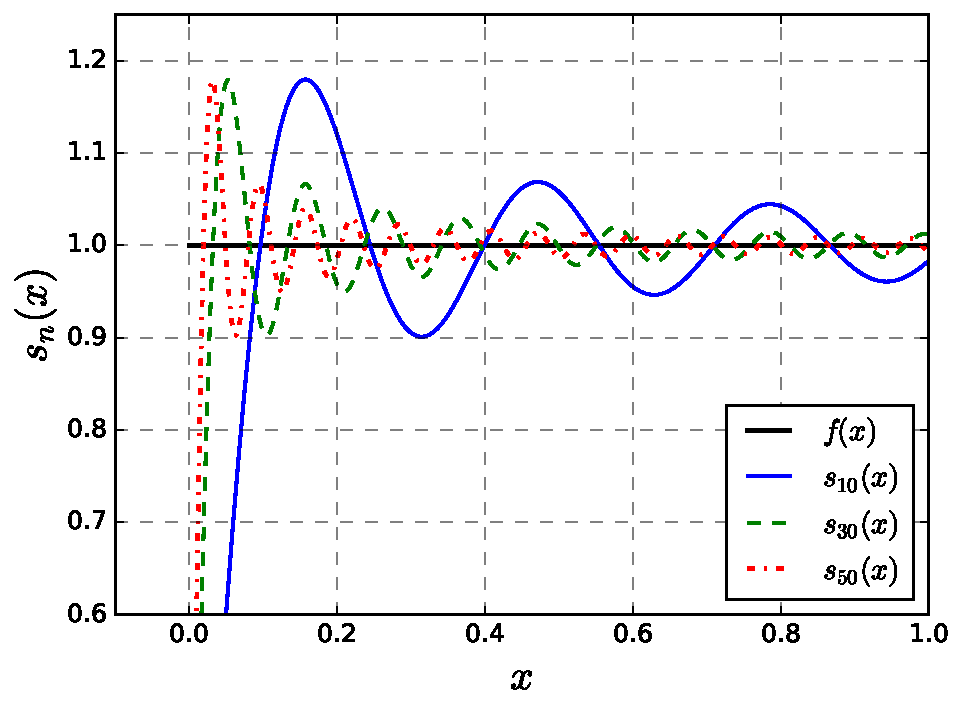
\includegraphics[scale = 0.65]{Figuras/FenomenoGibbs.pdf}
%     \caption{Fenómeno de Gibbs en la función signo para $n = 10,30,50$.}
%     \label{fig:GibssSign}
% \end{figure}

% Ilustremos este hecho con un análisis analítico de la función ya estudiada
% $$f(x) = \left\{ \begin{array}{cc}
%      -1,& - \pi \leq x < 0  \\
%      1,&   0 \leq x \leq \pi
% \end{array} \right. .$$

% Su serie de Fourier está dada por
% $$\sum_{n=1}^{\infty} \frac{4}{\pi} \frac{\sin[(2n-1)x]}{ (2n-1)}.$$

% Sea 
% $$s_n(x) = \frac{4}{\pi} \sum_{k=1}^n \frac{\sin[(2k-1)x]}{2k-1}$$

% su $n$-ésima suma parcial. Derivando y multiplicando por $\pi \sin(x)$, encontramos que 
% \begin{align*}
%    \pi (\sin x)s_n'(x) =4 \sin(x) \sum_{k=1}^n \cos[(2k-1)x] &= 4 \sum_{k=1}^n   \sin(x) \cos[(2k-1)x] \\
%    &= 4 \sum_{k=1}^n  \frac{1}{2}[\sin(x + (2k-1)x) + \sin(x - (2k-1)x)] \\
%    &= 2 \sum_{k=1}^n [\sin(2k x) - \sin([2k-2]x)] \\
%    &= 2 \sin(2nx).
% \end{align*}

% Luego, 
% \begin{equation*}
%   2 \sin(2nx_c) = 0 ~\Leftrightarrow~ x_c = \frac{m \pi}{2n}, \quad m \in \mathbb{Z}. 
% \end{equation*}

% Nos interesa encontrar el primer máximo de $s_n(x)$, así que tomaremos los valores $m = \pm 1$ de prueba, pues en $m = 0$ no se alcanza un máximo dado que $s_n(0) = 0$. Como $\sin(x_c) \neq 0$, para estos valores de $m$,  $s_n'(x_c) = 0$ y, en consecuencia, $x_c$ son los puntos críticos de $s_n$. 

% En la siguiente tabla se analizan los signos de $s_n'(x)$.

% \begin{figure}[H]
%     \centering
%     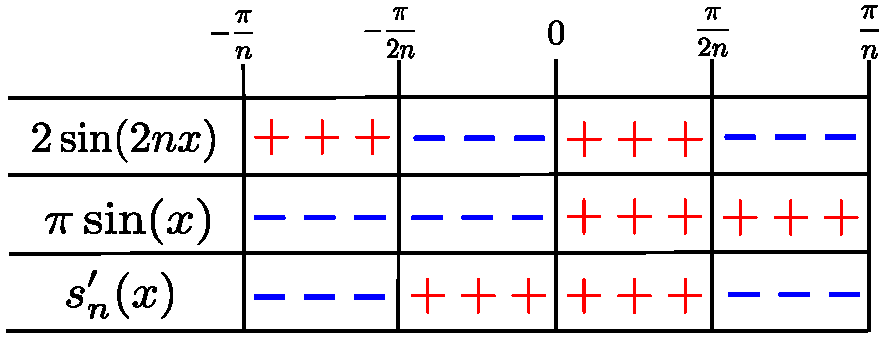
\includegraphics[scale = 0.62]{Figuras/EjemploGibbs.pdf}
%     \caption{Tabla con el análisis de signos de $s_n'(x)$ asociada a la función signo.}
% \end{figure}

% Por el criterio de la primera derivada, vemos que $s_n$ tiene un máximo en $x_n = \frac{\pi}{2n}$. El valor de ese máximo es
% $$s_n \left( \frac{\pi}{2n}\right) = \frac{4}{\pi} \sum_{k=1}^n \frac{\sin[(2k-1)\pi/2n]}{2k-1} = \frac{2}{\pi} \sum_{k=1}^n \frac{\sin[(2k-1)\pi /2n]}{(2k-1) \pi/2n} \left(\frac{\pi}{n} \right).$$

% Notemos que la sumatoria 
% $$ \sum_{k=1}^n \frac{\sin[(2k-1)\pi /2n]}{(2k-1) \pi/2n} \left(\frac{\pi}{n} \right)$$

% es una suma de Riemann para la función $\sin y/y$ en $[0,\pi]$ para la partición regular $0 = x_0 < x_1  <  \cdots< x_n =  \pi$ con $x_i = (\pi/n) i$, $i = 0,1, \dots, n$ y eligiendo el punto medio de cada intervalo $[x_{k-1},x_k]$,
% $$ \frac{x_{k-1} + x_k}{2} = (2k-1) \frac{\pi}{2n}, \quad  k = 1, \dots, n,$$

% para evaluar $\sin y/y$. Entonces, 
% $$\int_0^{\pi} \frac{\sin y}{y} \,dy \approx \frac{\pi}{2} s_n\left( \frac{\pi}{2n}\right).$$

% Como 
% $$\int_0^{\pi} \frac{\sin y}{y} \,dy ~~ \mbox{converge} ~\Rightarrow~ \lim_{n \to + \infty} s_n\left( \frac{\pi}{2n} \right) = \frac{2}{\pi} \int_0^{\pi} \frac{\sin y}{y} \,dy.$$

% Usando un método numérico de integración (o su calculadora de integrales favorita), 
% $$\int_0^{\pi} \frac{\sin y}{y} \,dy \approx 1.85193\dots$$

% Por lo tanto, 
% $$\lim_{n \to + \infty} s_n\left( \frac{\pi}{2n} \right) \approx 1.179.$$

% Así, las aproximaciones exceden el valor real de $f(0^+) = 1$ por $0.179$ o $8.95\%$ del salto de $f(0^-)$ a $f(0^+)$. 

% En general, se puede demostrar el siguiente teorema, debido a M. B$\hat{\mbox{o}}$cher \cite{Bôcher}:

% \begin{teorema}
% Sea $f$ una función de variable real, con período $2\pi$. Supongamos que $f$ y $f'$ son ambas continuas excepto para un número finito de discontinuidades de salto en el intervalo $[-\pi,\pi]$. Sea $s_n(x)$ la suma parcial de orden $n$ de Fourier. Entonces, en un punto $a$ de discontinuidad, las gráficas de las funciones $s_n(x)$ convergen al segmento vectical (ver figura \ref{Gibbs}) de longitud 
% $$L = \frac{2}{\pi} Si(\pi) |f(a^+) - f(a^-)| \approx 1.179 |f(a^+) - f(a^-)|$$

% centrada en el punto 
% $$\left(a, \frac{f(a^+) + f(a^-)}{2} \right),$$

% donde $Si(x)$ es la función seno integral definida por
% $$Si(x) = \int_0^x \frac{\sin t}{t} \,dt.$$
% \end{teorema}

% \begin{figure}[H]
%     \centering
%     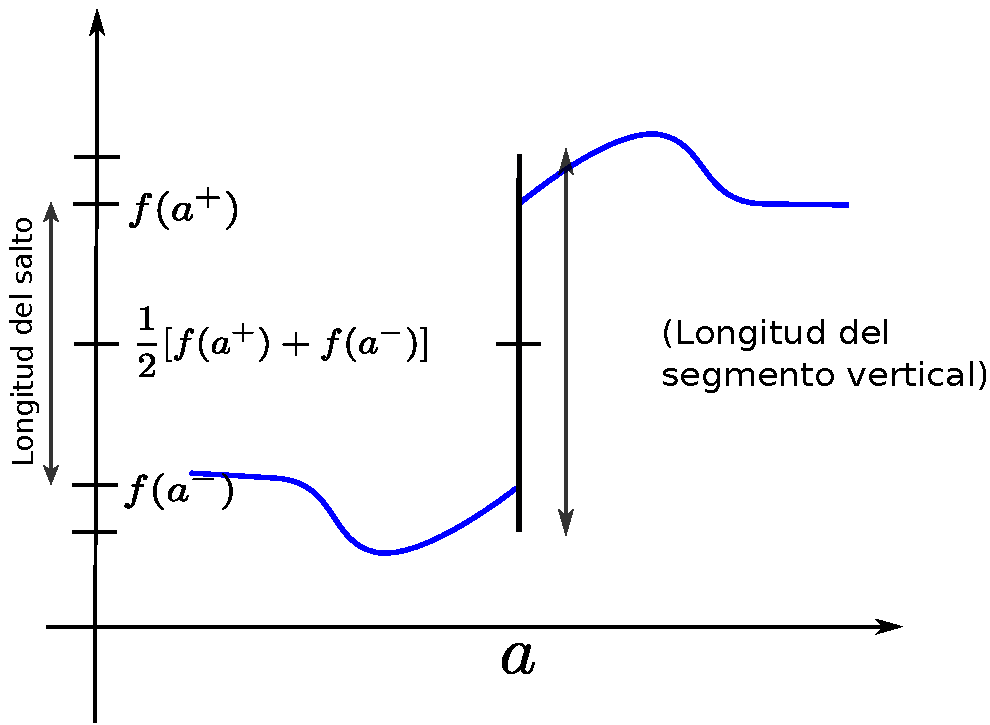
\includegraphics[scale = 0.51]{Figuras/Gibbs.pdf}
%     \caption{Fenómeno de Gibbs en un punto de discontinuidad. Adaptado de \cite{UFRO}, pág. 202.}
%     \label{Gibbs}
% \end{figure}